\documentclass[border=5pt]{standalone}
\usepackage{tikz,graphicx,amsmath,amssymb,xcolor}\usepackage{fontspec,xeCJK}\setmainfont{Helvetica}\setCJKmainfont{PingFang SC}
\usetikzlibrary{arrows.meta}
\definecolor{ink}{HTML}{203D46}\definecolor{teal}{HTML}{277A80}\definecolor{pale}{HTML}{EFF6F5}\definecolor{warm}{HTML}{F6ECDD}\definecolor{training}{HTML}{BB7347}
\begin{document}\begin{tikzpicture}[x=1mm,y=1mm,font=\fontsize{11}{14}\selectfont,text=ink]
\path[use as bounding box] (-11,0) rectangle (120,260);
\node[anchor=north west,font=\bfseries\fontsize{16}{19}\selectfont] at (3,258) {RT-1：一张图走完整条链};
\node[anchor=north west,text width=98mm,font=\fontsize{10}{13}\selectfont] at (3,248) {运行：$A\to B\to C\to E$，新观测回 A。训练：D 的示范监督 C；语言先参与视觉提取。};
\fill[pale,rounded corners=2mm] (1,191) rectangle (104,232);
\node[anchor=north west,text=teal,font=\bfseries\fontsize{12}{15}\selectfont] at (4,230) {A 看六帧，听一句 · §5.1};
\node[anchor=north west,text width=66mm,inner sep=0] at (4,222) {$6\times300\times300\times3$ 图像\\语言 $e\in\mathbb R^{512}$ 调制 FiLM\\EfficientNet-B3：每帧\\$9\times9\times512$ 特征};
\node[anchor=center,inner sep=0] at (88,208) {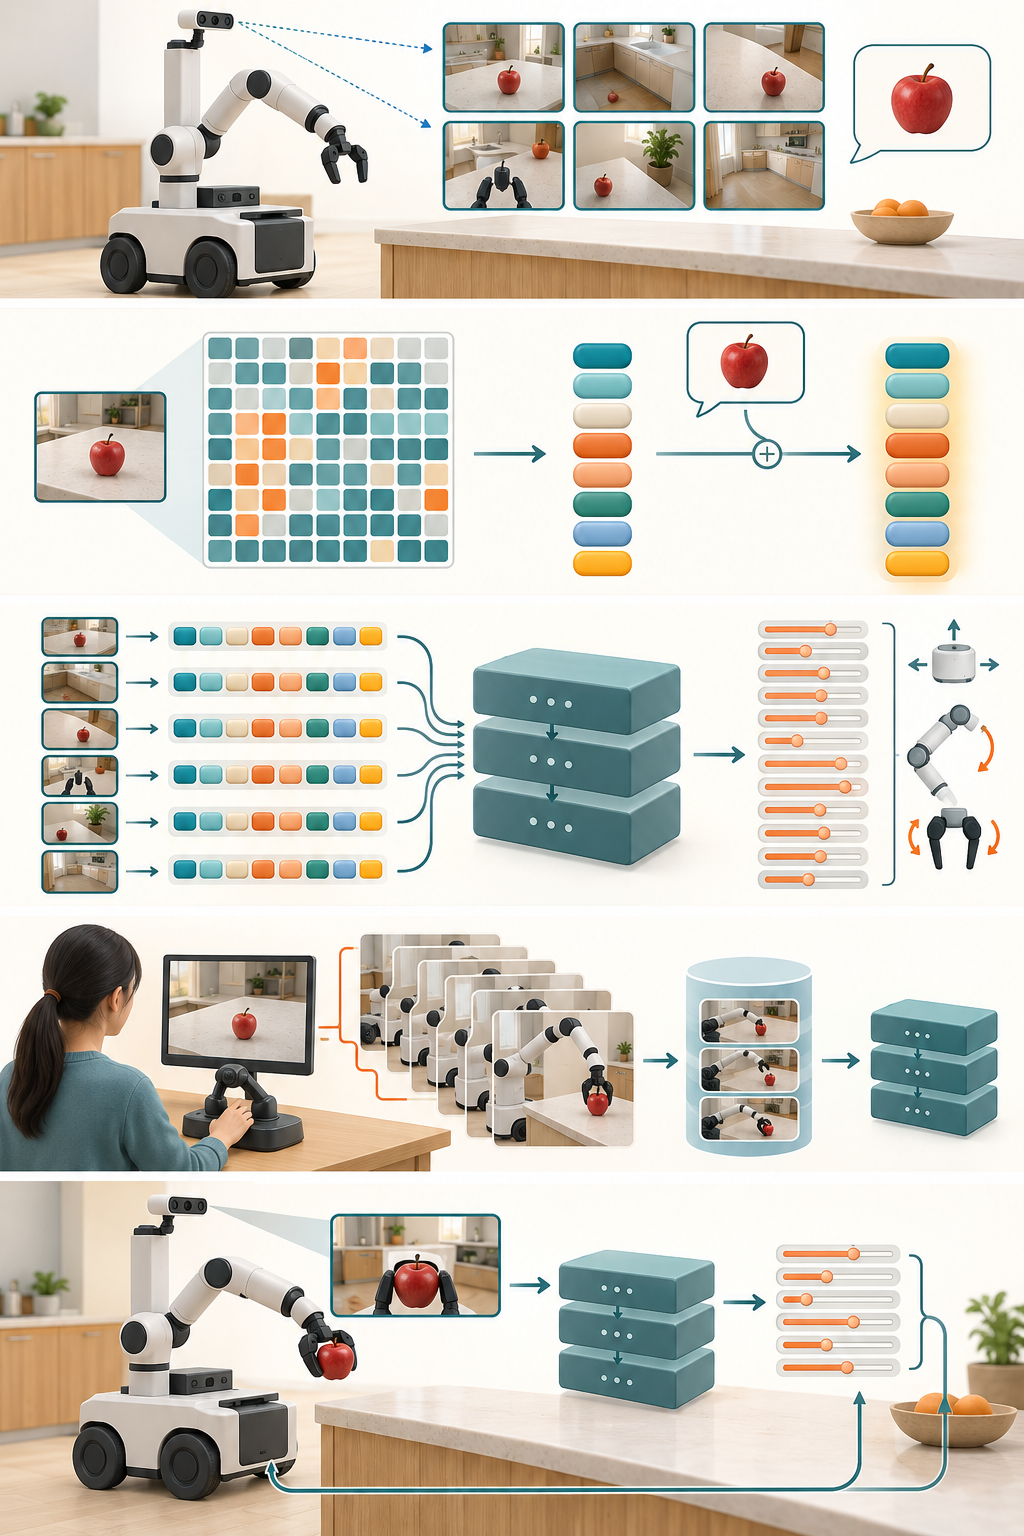
\includegraphics[width=26mm,height=31mm,keepaspectratio,viewport=0 1236 1024 1536,clip]{rt1-imagegen-draft.png}};
\draw[-{Latex[length=2mm]},teal,line width=.7pt] (52.5,190.5) -- (52.5,187);
\fill[pale,rounded corners=2mm] (1,145) rectangle (104,186);
\node[anchor=north west,text=teal,font=\bfseries\fontsize{12}{15}\selectfont] at (4,184) {B 视觉压缩 · §5.1};
\node[anchor=north west,text width=66mm,inner sep=0] at (4,176) {每帧 $81\times512$\\TokenLearner 加权汇聚\\每帧 $8\times512$\\六帧合为 $48\times512$};
\node[anchor=center,inner sep=0] at (88,162) {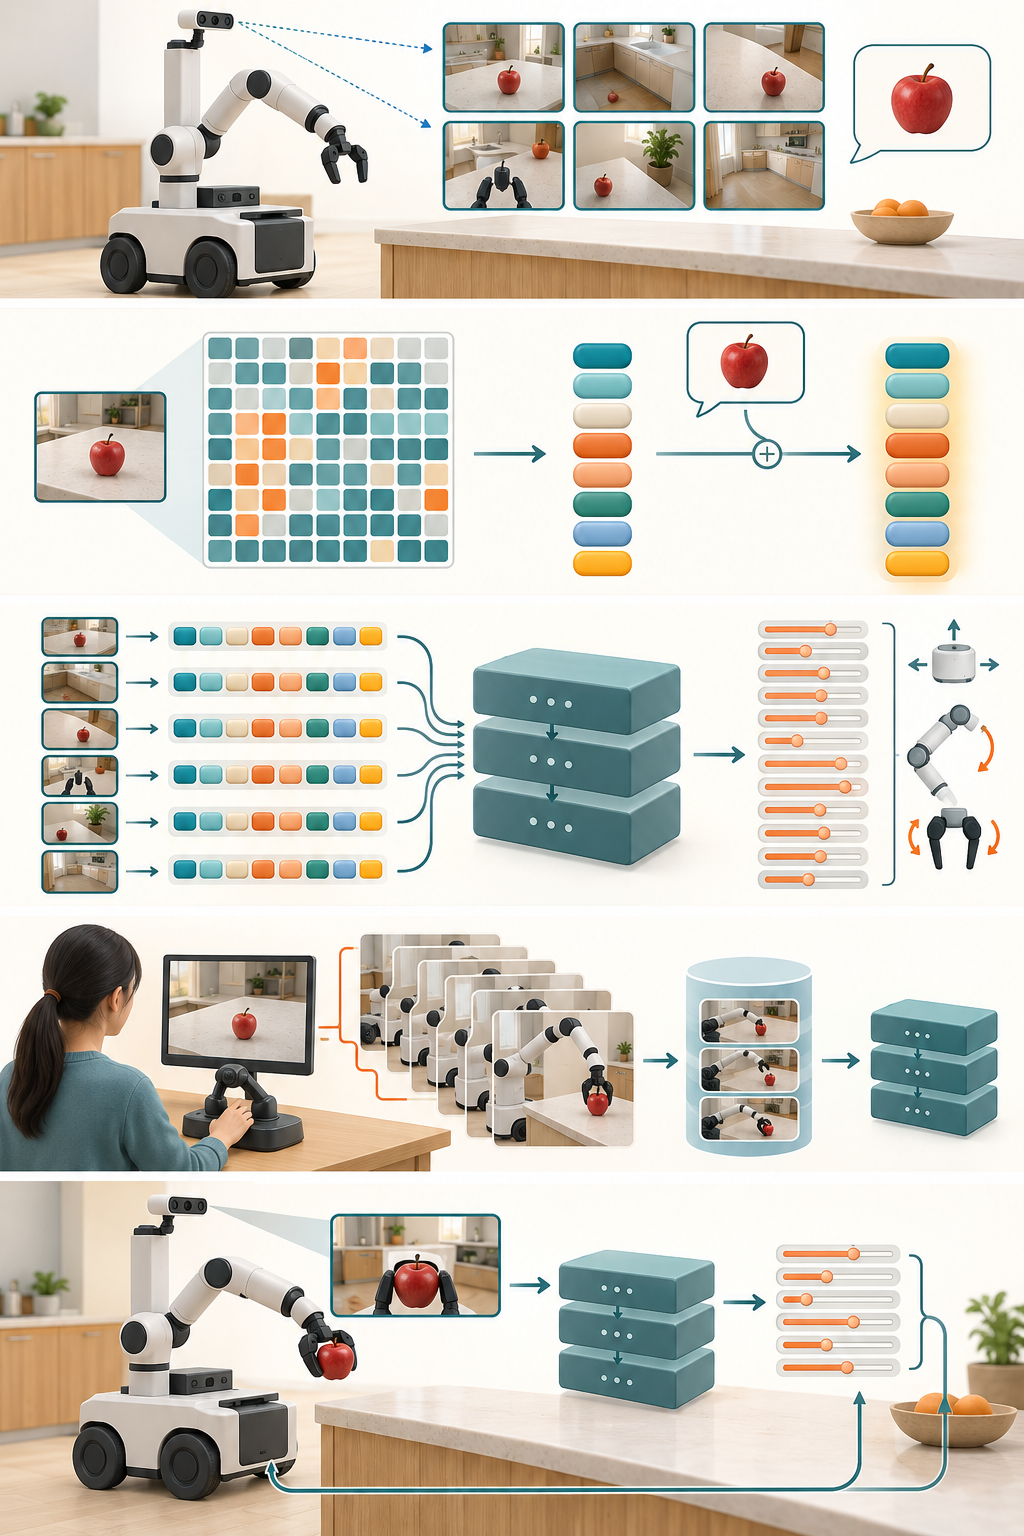
\includegraphics[width=26mm,height=31mm,keepaspectratio,viewport=0 940 1024 1226,clip]{rt1-imagegen-draft.png}};
\draw[-{Latex[length=2mm]},teal,line width=.7pt] (52.5,144.5) -- (52.5,141);
\fill[pale,rounded corners=2mm] (1,99) rectangle (104,140);
\node[anchor=north west,text=teal,font=\bfseries\fontsize{12}{15}\selectfont] at (4,138) {C 从历史到动作 · §5.1};
\node[anchor=north west,text width=66mm,inner sep=0] at (4,130) {位置编码 + 8 层 Transformer\\11 个动作分量\\连续量离散为 256 档\\本版不逐分量自回归生成};
\node[anchor=center,inner sep=0] at (88,116) {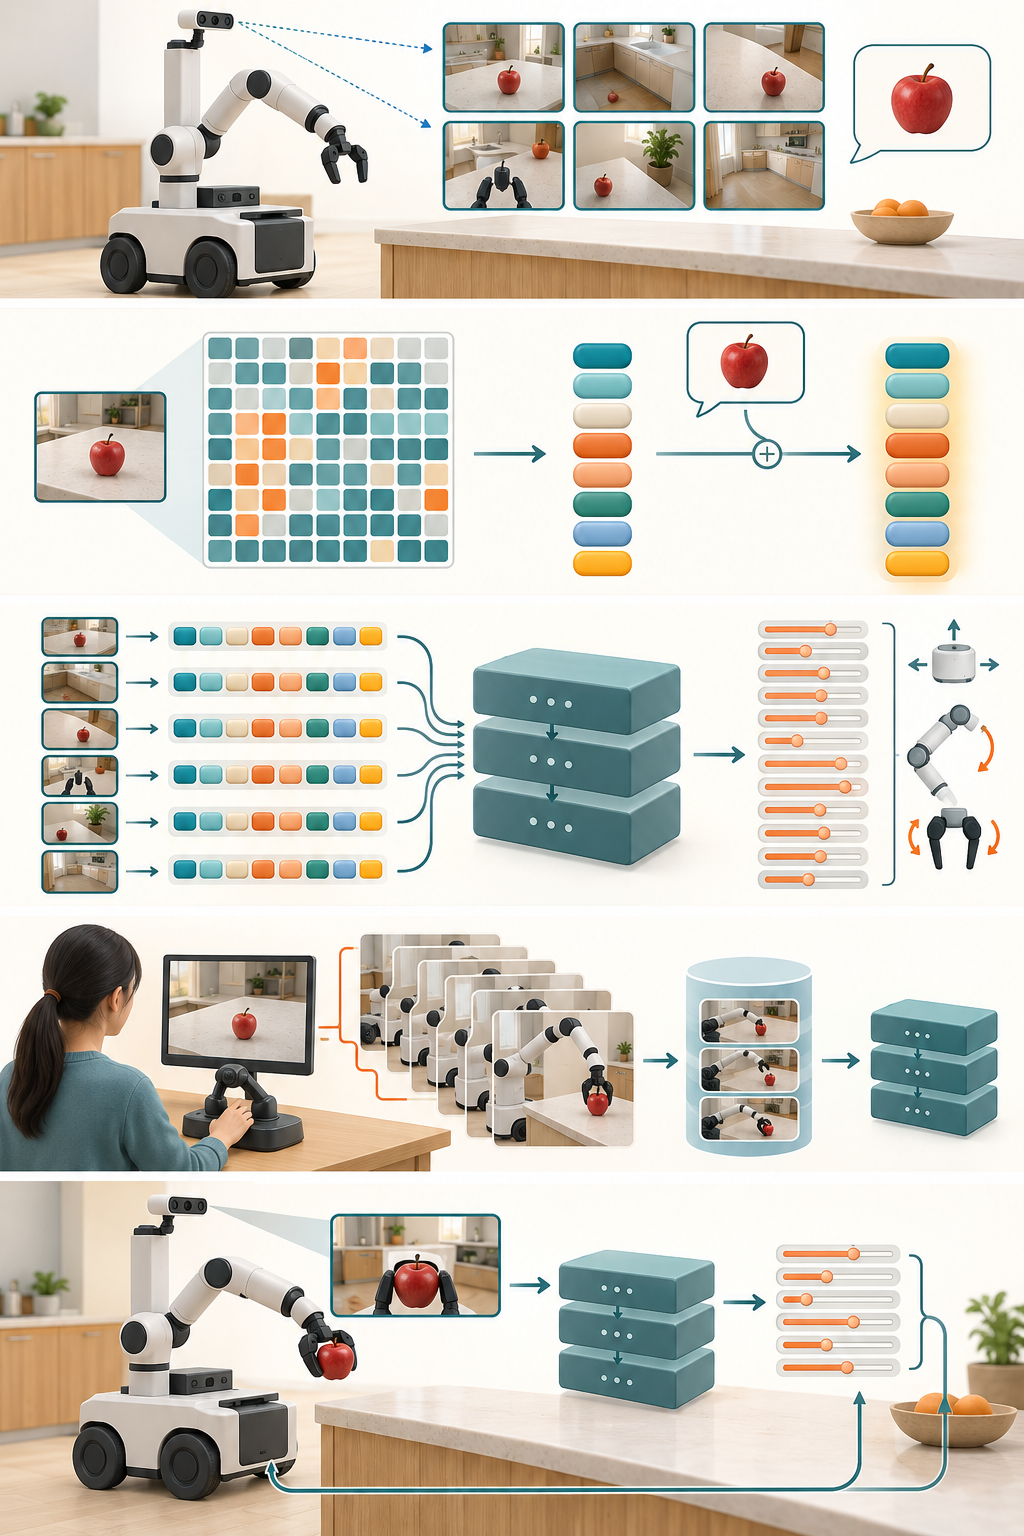
\includegraphics[width=26mm,height=31mm,keepaspectratio,viewport=0 634 1024 926,clip]{rt1-imagegen-draft.png}};

\fill[warm,rounded corners=2mm] (1,53) rectangle (104,94);
\node[anchor=north west,text=teal,font=\bfseries\fontsize{12}{15}\selectfont] at (4,92) {D 示范怎样教 · §5.2};
\node[anchor=north west,text width=66mm,inner sep=0] at (4,84) {13 台机器人，约 13 万回合\\语言 / 图像 / 人类动作配对\\动作档位交叉熵\\梯度更新视觉编码器与策略};
\node[anchor=center,inner sep=0] at (88,70) {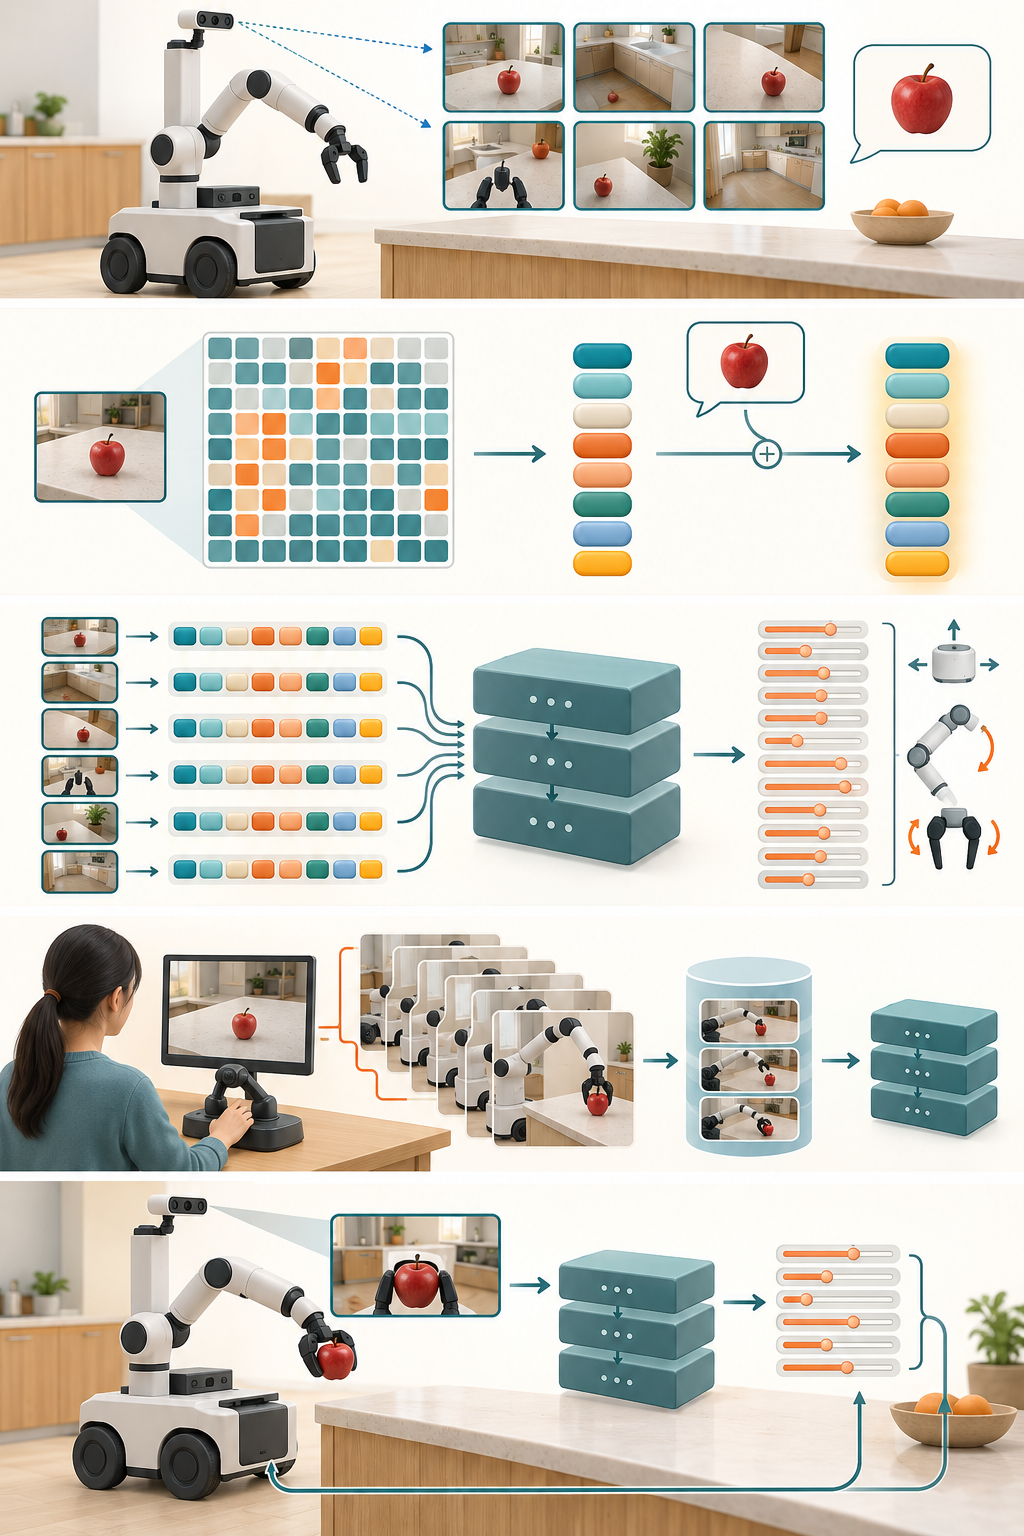
\includegraphics[width=26mm,height=31mm,keepaspectratio,viewport=0 363 1024 618,clip]{rt1-imagegen-draft.png}};

\fill[pale,rounded corners=2mm] (1,7) rectangle (104,48);
\node[anchor=north west,text=teal,font=\bfseries\fontsize{12}{15}\selectfont] at (4,46) {E 执行再看 · §6};
\node[anchor=north west,text width=66mm,inner sep=0] at (4,38) {动作解码 $\rightarrow$ 机械臂 / 底盘\\3 Hz 闭环，刷新六帧历史\\测新任务、干扰和新背景\\跨数据来源比较迁移};
\node[anchor=center,inner sep=0] at (88,24) {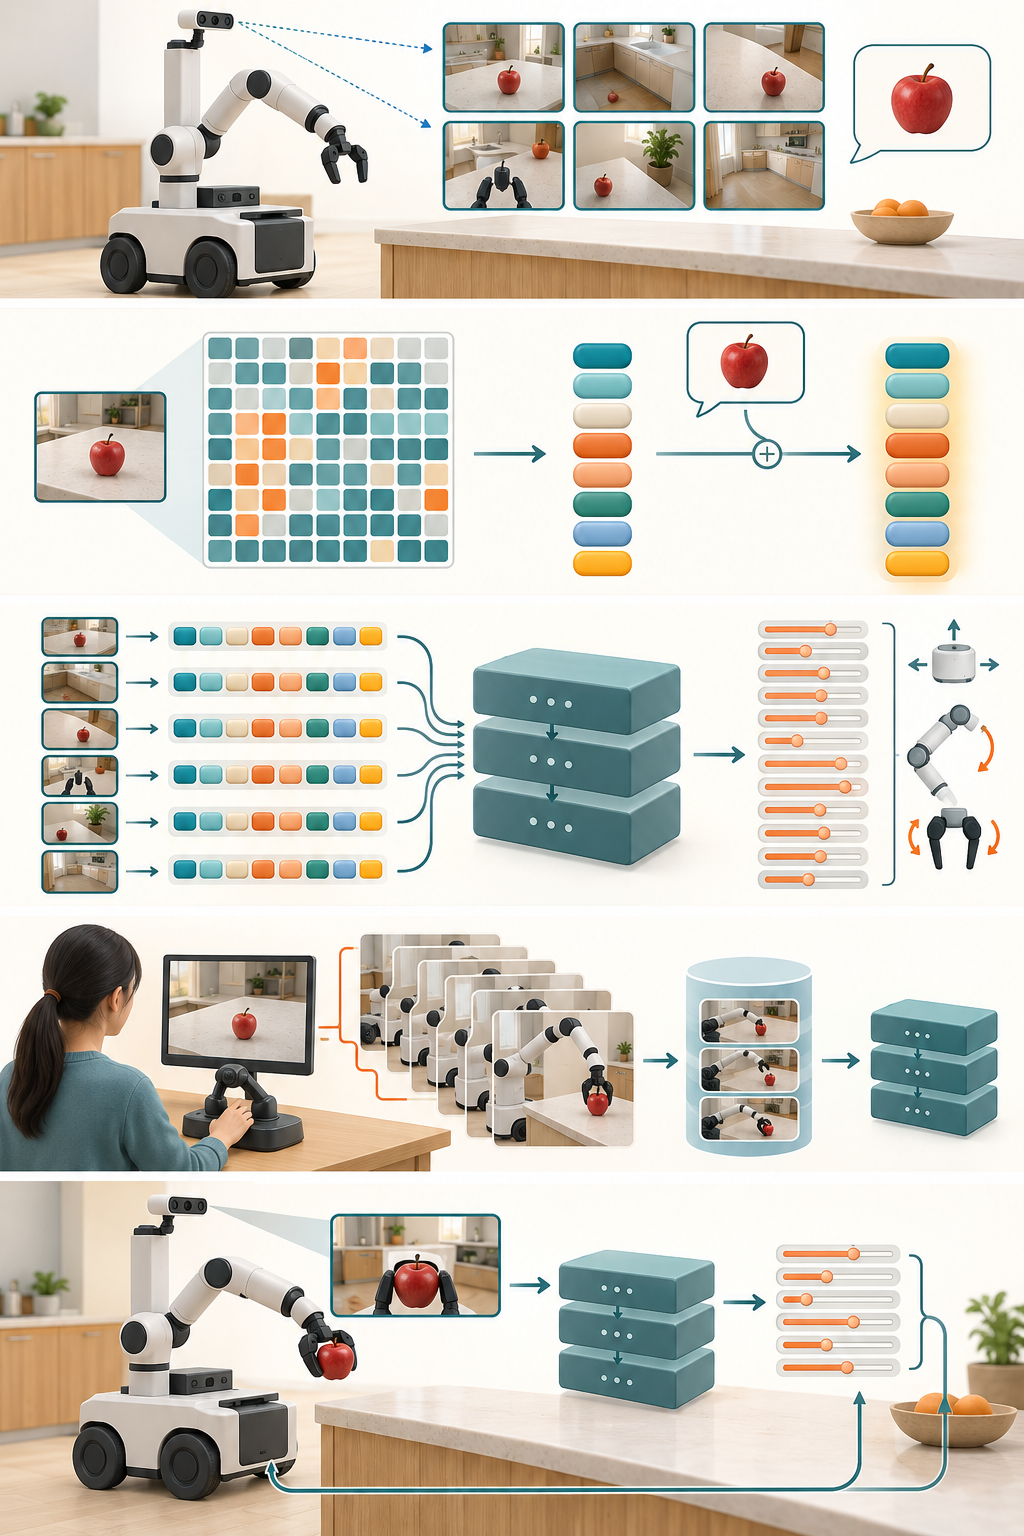
\includegraphics[width=26mm,height=31mm,keepaspectratio,viewport=0 0 1024 355,clip]{rt1-imagegen-draft.png}};
\draw[-{Latex[length=2mm]},teal,line width=.8pt] (104,119) -- (111,119) -- (111,28) -- (104,28);
\node[rotate=90,text=teal,font=\fontsize{9}{11}\selectfont,fill=white,inner sep=1pt] at (114,74) {C 到 E：运行时动作};
\draw[-{Latex[length=2mm]},training,dashed,line width=.9pt] (52.5,94) -- (52.5,99);
\node[text=training,font=\fontsize{8}{10}\selectfont,anchor=west] at (56,96.5) {D 到 C：训练监督};
\draw[-{Latex[length=2mm]},teal,line width=.6pt] (1,28) -- (-5,28) -- (-5,211) -- (1,211);
\node[rotate=90,text=teal,font=\fontsize{8}{10}\selectfont,fill=white,inner sep=1pt] at (-7,119) {执行后刷新观察};
\end{tikzpicture}\end{document}